% !TeX program = xelatex
% C3 midterm defense – unified deck: ZBY theory + RQ1 + RQ3 + RQ2.
\PassOptionsToPackage{quiet}{fontspec}
\PassOptionsToPackage{dvipsnames}{xcolor}
\PassOptionsToPackage{fontset=fandol}{ctex}
\documentclass[10pt,aspectratio=169]{beamer}

\usepackage{zju_beamer}
\usepackage{booktabs}
\usepackage{tabularx}
\usepackage{array}
\usepackage{mathtools}

\graphicspath{{./figures/}}
\zjusectioncolor{blue}
\setbeamertemplate{navigation symbols}{}

\definecolor{ZJUBlue}{RGB}{0,63,136}
\definecolor{ZJULight}{RGB}{236,244,252}
\definecolor{ZJUGreen}{RGB}{0,125,117}
\definecolor{WarmGray}{RGB}{90,90,90}

\newcommand{\key}[1]{\textcolor{ZJUBlue}{\textbf{#1}}}
\newcommand{\good}[1]{\textcolor{ZJUGreen}{\textbf{#1}}}
\newcommand{\R}{\mathbb{R}}
\newcommand{\E}{\mathbb{E}}
\newcommand{\argmax}{\operatorname*{arg\,max}}

\title[C3：数据增强 AutoML 定价]{数据增强 AutoML 市场中的最优定价}
\subtitle{论文理论解读 · 实验复现 · 机制讨论}
\author[张博渊、林润铎、彭博宇]{张博渊、林润铎、彭博宇}
\institute[数据要素市场]{数据要素市场课程 · 中期答辩\\参考论文：\textit{Optimal Pricing for Data-Augmented AutoML Marketplaces}}
\date{2026 年 7 月 18 日}

\AtBeginSection[]{
  \begin{frame}[plain,noframenumbering]
    \vfill
    \centering
    {\color{WarmGray}\large 第 \insertsectionnumber{} 部分}\par
    \vspace{0.8em}
    {\color{ZJUBlue}\bfseries\LARGE \insertsectionhead}\par
    \vspace{0.7em}
    {\color{ZJUBlue}\rule{0.34\textwidth}{1.2pt}}
    \vfill
  \end{frame}
}

\begin{document}

% ============================== Title ==============================

\begin{frame}
  \titlepage
\end{frame}

\begin{frame}{目录}
  \tableofcontents[hideallsubsections]
\end{frame}

\begin{frame}{理论部分完成的工作}
  \begin{columns}[T,onlytextwidth]
    \begin{column}{0.31\textwidth}
      \begin{block}{机制重构}
        将分散在论文各节的模型整理为\key{轨迹、停止、定价、学习}四个环节。
      \end{block}
    \end{column}
    \begin{column}{0.31\textwidth}
      \begin{block}{结论提炼}
        从 DP、MILP 与学习理论中提炼四条可直接解释和检验的结论。
      \end{block}
    \end{column}
    \begin{column}{0.31\textwidth}
      \begin{block}{边界识别}
        明确结论成立所需的性能动态、买方偏好与信息条件。
      \end{block}
    \end{column}
  \end{columns}
  \vspace{0.8em}
\end{frame}

% ============================== 研究问题 ==============================

\section{研究问题}

\begin{frame}{数据本身值多少钱不是主要问题，而是模型增益值多少钱}
  \begin{columns}[T,onlytextwidth]
    \begin{column}{0.47\textwidth}
      \begin{block}{直接售卖数据的错配}
        \begin{itemize}
          \item 数据价值\key{依赖具体任务}，买方事前难判断是否有用；
          \item AutoML 按计算时间收费，买方可能为\key{无效搜索}承担成本；
          \item 不同买方对同一性能提升有不同支付意愿。
        \end{itemize}
      \end{block}
    \end{column}
    \begin{column}{0.48\textwidth}
      \begin{block}{论文的定价对象}
        \centering
        \large
        \[
          \Delta q=q(C\leftarrow D\Join A)-q(C_0\leftarrow D)
        \]
        \normalsize
        数据增强与模型搜索共同产生的\key{工具性价值}
      \end{block}
      \begin{alertblock}{机制载体}
        平台预先公布统一价格曲线 $x(q)$，按买方最终购买的性能档位收费。
      \end{alertblock}
    \end{column}
  \end{columns}
\end{frame}

% ============================== 机制与结论 ==============================

\section{机制与结论}

\begin{frame}{平台把数据发现、模型搜索与定价接成一个闭环}
  \begin{itemize}
    \item 买方提交任务、初始训练数据和评估方式；平台从外部数据池中搜索增广特征与模型。
    \item 发现引擎持续输出性能轨迹，定价引擎将其转换为“\key{性能-价格}”菜单。
  \end{itemize}
  \vspace{0.25em}
  \begin{center}
    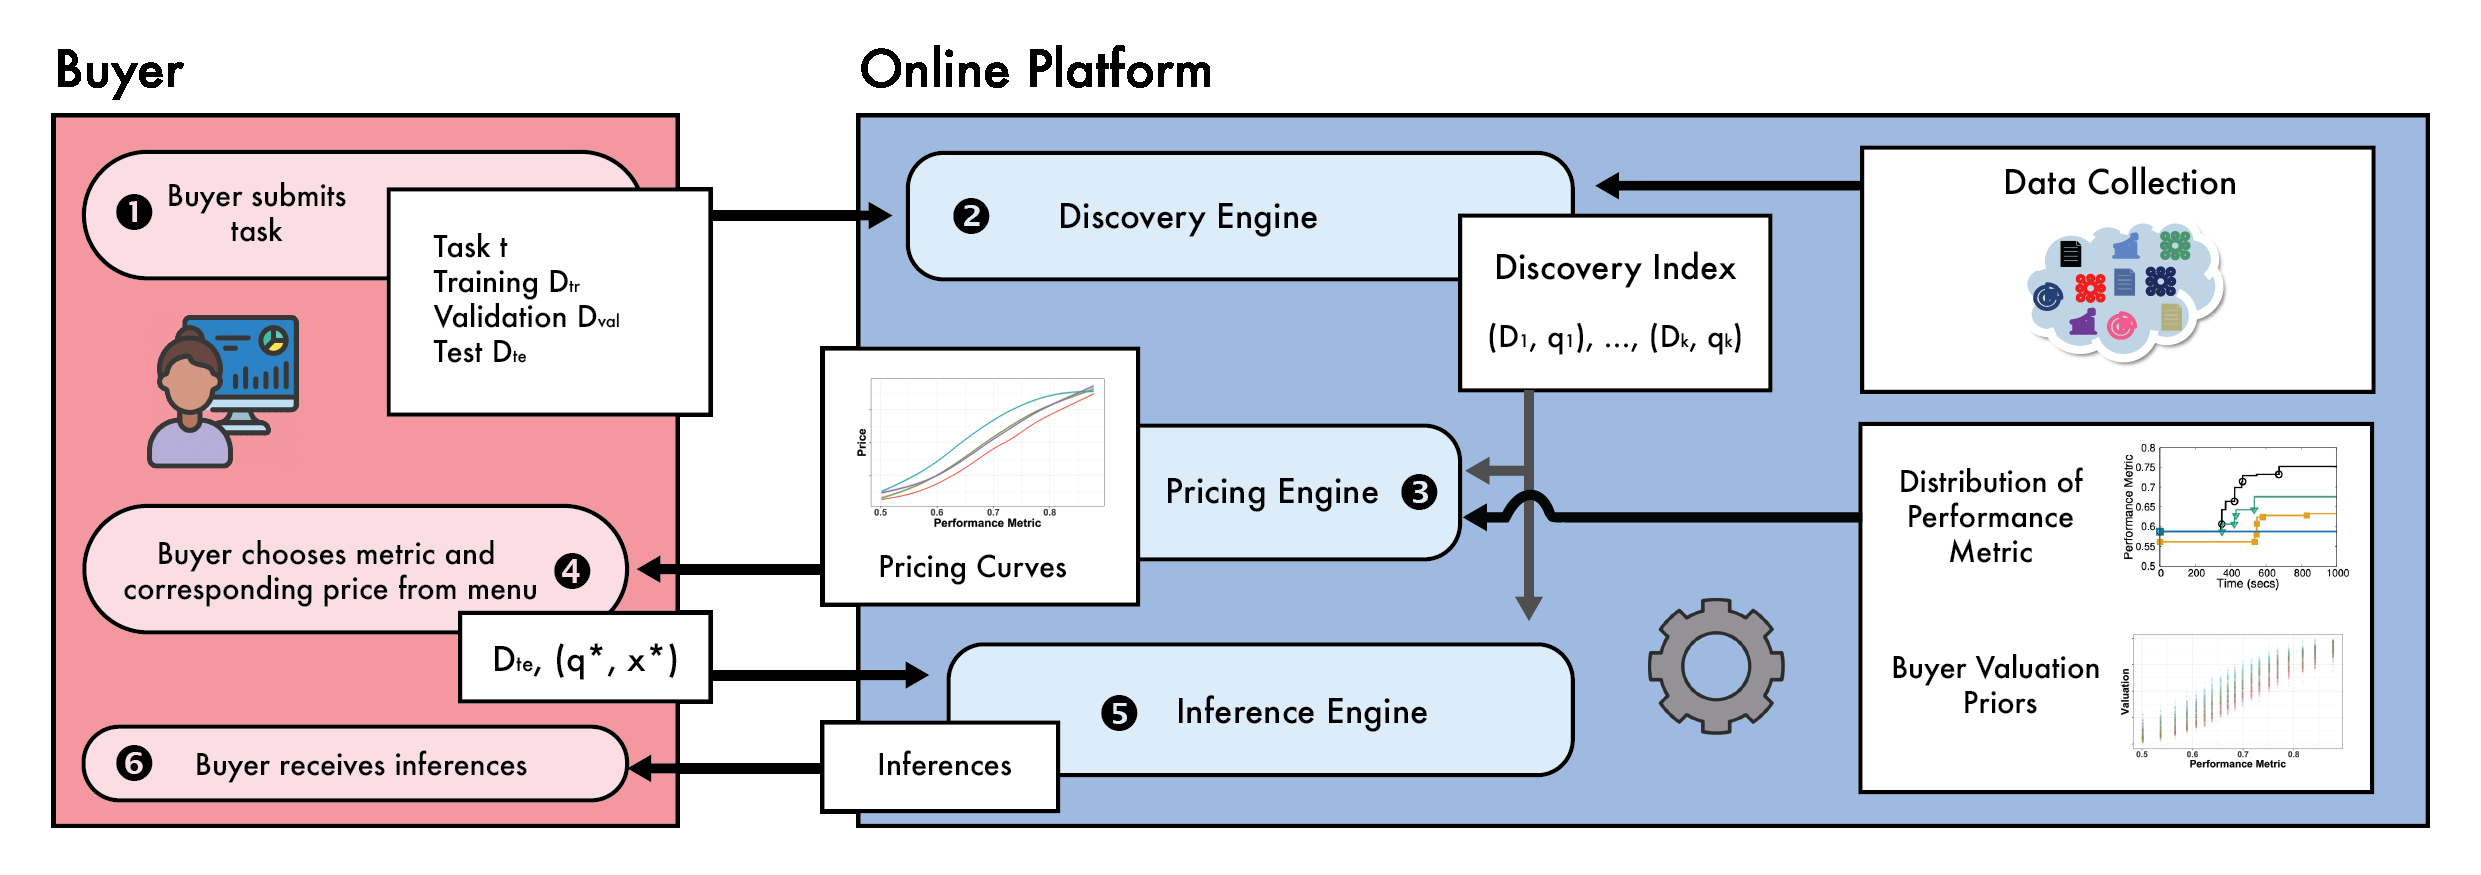
\includegraphics[width=0.88\linewidth]{paper_architecture.png}
  \end{center}
\end{frame}

\begin{frame}{公开价格曲线同时处理性能、偏好与搜索成本}
  \small
  \renewcommand{\arraystretch}{1.18}
  \begin{tabularx}{\linewidth}{>{\bfseries\color{ZJUBlue}}l X}
    \toprule
    符号                & 在机制中的作用                          \\
    \midrule
    $\mathcal Q, q_t$ & 离散化的模型性能集合与当前观测性能。               \\
    $P^t(q'\mid q)$   & 性能从本期到下一期的搜索动态。                  \\
    $c,T$             & 每期真实搜索成本与最长搜索期数。                 \\
    $\theta\sim\mu$   & 买方类型及其先验；$v^\theta(q)$ 表示对性能的价值。 \\
    $x(q)$            & 平台面向所有买方公开的性能价格。                 \\
    \bottomrule
  \end{tabularx}
  \vspace{0.2em}
  \begin{block}{买方只比较一件事}
    \centering
    \large
    $\text{净效用}=\text{性能价值}-\text{价格}-\text{搜索成本}$
  \end{block}
\end{frame}

\begin{frame}{买方通过停止时点表达自己的支付意愿}
  \begin{columns}[T,onlytextwidth]
    \begin{column}{.225\textwidth}
      \begin{block}{1. 进入前}
        平台公开价格、成本与性能演化信息。
      \end{block}
    \end{column}
    \begin{column}{.225\textwidth}
      \begin{block}{2. 搜索中}
        每期看到最新性能，保留已经出现的优质档位。
      \end{block}
    \end{column}
    \begin{column}{.225\textwidth}
      \begin{block}{3. 自主决策}
        比较立即停止与继续搜索的期望收益。
      \end{block}
    \end{column}
    \begin{column}{.225\textwidth}
      \begin{block}{4. 退出或购买}
        选择历史上净效用最高的档位，也可以不购买。
      \end{block}
    \end{column}
  \end{columns}
  \vspace{0.8em}
  \begin{alertblock}{机制性质}
    平台不要求买方主动报告类型；不同支付意愿通过\key{停止时点与购买档位}自然表现出来。
  \end{alertblock}
\end{frame}

\begin{frame}{结论 1：买方遵循“立即停止还是继续搜索”的阈值规则}
  \begin{columns}[T,onlytextwidth]
    \begin{column}{0.53\textwidth}
      \centering
      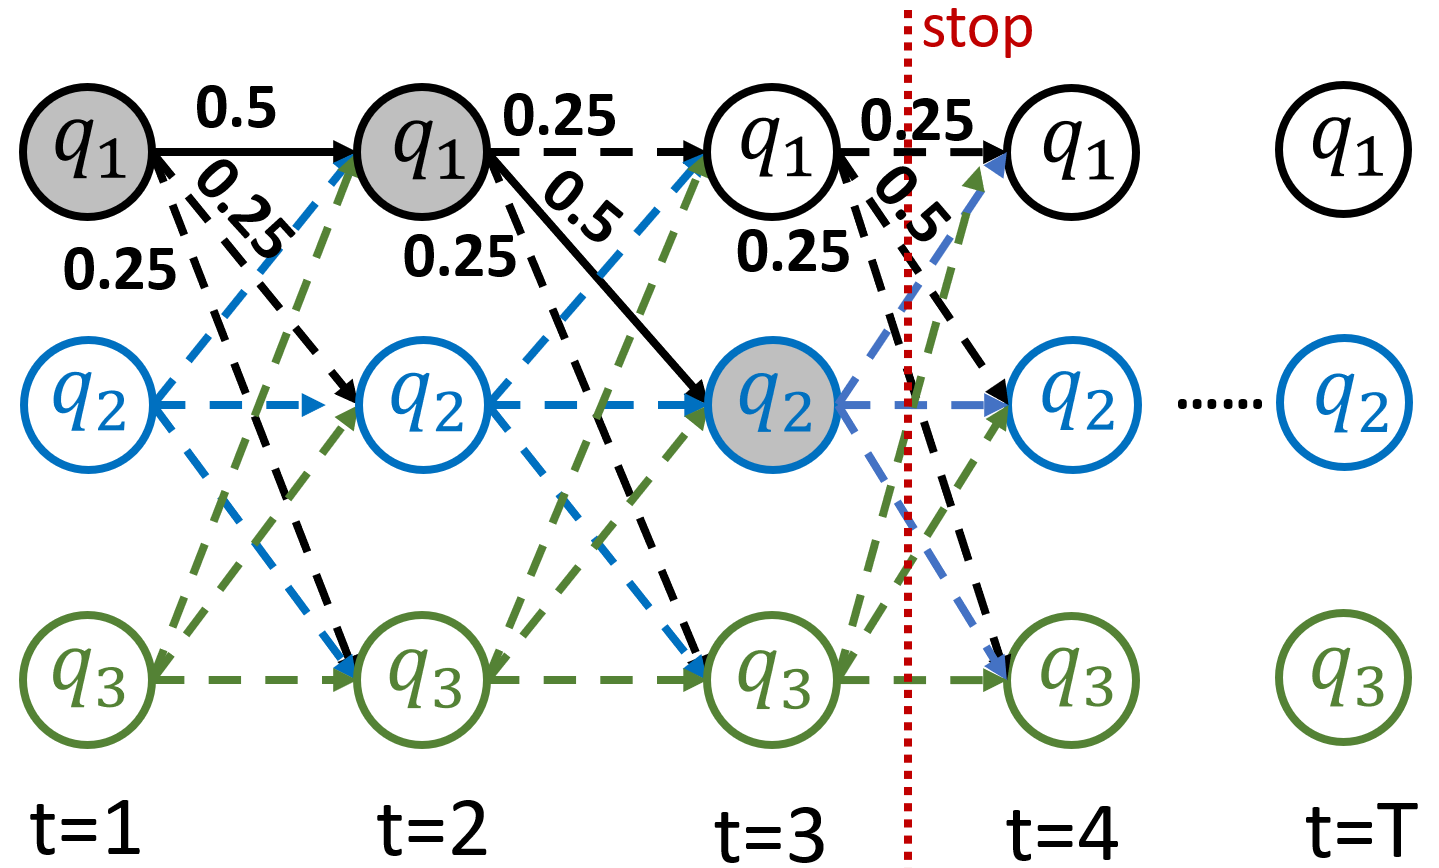
\includegraphics[width=0.96\linewidth]{paper_markov.png}
    \end{column}
    \begin{column}{0.42\textwidth}
      \begin{block}{这是相关收益的 Pandora's Box}
        \begin{itemize}
          \item 下一期性能依赖当前 $q_t$；
          \item 决策需要记住历史最佳净效用；
          \item 搜索存在有限期限与逐期成本。
        \end{itemize}
      \end{block}
      \begin{alertblock}{结论}
        若\key{立即停止效用}不低于\key{继续搜索的期望效用}，买方停止；否则继续。
      \end{alertblock}
    \end{column}
  \end{columns}
\end{frame}

\begin{frame}{结论 2：三个状态量足以计算买方的最优停止}
  \begin{columns}[T,onlytextwidth]
    \begin{column}{0.31\textwidth}
      \begin{block}{历史最好 $q_1$}
        到目前为止，净效用最高的性能档位。
      \end{block}
    \end{column}
    \begin{column}{0.31\textwidth}
      \begin{block}{当前性能 $q_2$}
        决定下一期性能的条件分布。
      \end{block}
    \end{column}
    \begin{column}{0.31\textwidth}
      \begin{block}{当前时间 $t$}
        决定剩余期限与累计搜索成本。
      \end{block}
    \end{column}
  \end{columns}
  \vspace{0.8em}
  \begin{alertblock}{命题 4.1 的结论}
    动态规划只需遍历 $|\mathcal Q|^2T$ 个状态，最优停止策略可在
    \good{$O(|\mathcal Q|^2T)$} 时间内求得。

    平台无需枚举所有搜索历史，只需维护这三个状态量，就能预测买方的最优响应。
  \end{alertblock}
\end{frame}

\begin{frame}{结论 3：把买方选择写入 MILP，平台价格即可计算}
  \begin{columns}[T,onlytextwidth]
    \begin{column}{0.45\textwidth}
      \begin{block}{原问题是双层优化}
        \begin{itemize}
          \item 平台先选择价格曲线；
          \item 买方随后选择净效用最高的档位；
          \item 平台收入取决于买方的离散选择。
        \end{itemize}
      \end{block}
    \end{column}
    \begin{column}{0.50\textwidth}
      \begin{block}{MILP 的转写思路}
        \begin{itemize}
          \item $x$ 表示公开价格；
          \item $z$ 表示买方选择哪个档位；
          \item $a$ 记录最大净效用；
          \item $y$ 记录该选择带来的实际收入。
        \end{itemize}
      \end{block}
    \end{column}
  \end{columns}
  \vspace{0.55em}
  \begin{alertblock}{结论}
    通过 Big-$M$ 约束把“买方最优选择”和“平台收入”同时编码后，可直接用标准 MILP 求解器输出整条价格曲线。
  \end{alertblock}
\end{frame}

\begin{frame}{结论 4：有限轨迹足以学习近优价格}
  \begin{alertblock}{定理 4.2 及其结论}
    在买方价值有界、发现成本相对价值可忽略时，只要样本量满足
    \[
      m\ge \frac{b^2}{2\varepsilon^2}\ln\frac{2}{\delta},
    \]
    学到的价格曲线以至少 $1-2\delta$ 的概率达到距最优收入不超过 $\varepsilon$ 的水平。
  \end{alertblock}
  \begin{columns}[T,onlytextwidth]
    \begin{column}{0.31\textwidth}
      \begin{block}{精度代价}
        $\varepsilon$ 减半，所需样本量约增至四倍。
      \end{block}
    \end{column}
    \begin{column}{0.31\textwidth}
      \begin{block}{数据要求}
        只需采样真实性能轨迹，不必写出完整转移矩阵。
      \end{block}
    \end{column}
    \begin{column}{0.31\textwidth}
      \begin{block}{机制含义}
        价格曲线不仅可计算，而且能从有限历史任务中学习。
      \end{block}
    \end{column}
  \end{columns}
\end{frame}

\begin{frame}{停止行为既能学习买方先验，也限制估计误差的损失}
  \begin{columns}[T,onlytextwidth]
    \begin{column}{0.47\textwidth}
      \begin{block}{先验如何学习}
        \begin{enumerate}
          \item 观察买方在什么性能与时间停止；
          \item 比较不同类型产生该行为的可能性；
          \item 反复交互后更新类型分布。
        \end{enumerate}
      \end{block}
    \end{column}
    \begin{column}{0.48\textwidth}
      \begin{alertblock}{定理 5.2 的结论}
        若买方先验 $\mu$ 与性能动态 $P$ 的估计误差均为 $\varepsilon$ 量级，则平台收入损失仅为
        \[
          O(\varepsilon).
        \]
      \end{alertblock}
    \end{column}
  \end{columns}
  \vspace{0.6em}
  \begin{block}{前提}
    不同买方类型必须在某些价格下产生可区分的停止分布，否则仅凭行为无法识别类型。
  \end{block}
\end{frame}

\begin{frame}{发现引擎每轮只训练一个模型，持续输出可定价轨迹}
  \begin{columns}[T,onlytextwidth]
    \begin{column}{0.4\textwidth}
      \begin{block}{为什么不能穷举}
        增广子集与模型的组合数量快速膨胀；每轮测试全部模型会让搜索成本无法接受。
      \end{block}
    \end{column}
    \begin{column}{0.55\textwidth}
      \begin{alertblock}{联合发现算法}
        \begin{enumerate}
          \item 用 Metam 聚类并选择候选增广；
          \item 将模型视作 Exp3 的不同臂；
          \item 每轮只采样并训练\key{一个模型}；
          \item 用当前性能更新模型权重。
        \end{enumerate}
      \end{alertblock}
    \end{column}
  \end{columns}
  \vspace{0.55em}
  \begin{block}{与定价机制的接口}
    算法具备 anytime 性质：每轮输出一个 $q_t$，买方可随时停止；性能序列正是停止策略与价格学习所需的轨迹。
  \end{block}
\end{frame}

\begin{frame}{四条建模边界决定理论结论能否成立}
  \begin{enumerate}
    \item \key{性能动态：}$\mathcal Q$ 有限离散，未来性能只依赖当前性能与时间；动态可公开或估计。
    \item \key{买方偏好：}类型空间有限、价值有界；不同类型的停止行为具有可识别性。
    \item \key{价格形式：}平台对所有买方公布同一条按性能收费的价格曲线，不依赖主动报告。
    \item \key{计算假设：}PAC 保证要求发现成本相对价值可忽略；一般误差的收入影响由鲁棒性结论控制。
  \end{enumerate}
  \vspace{0.55em}
  \begin{alertblock}{范围边界}
    论文主要解决“买方停止决策 + 平台收入最优定价”；上游数据供应者之间如何分配收入不在核心模型内。
  \end{alertblock}
\end{frame}

% ============================== RQ1 ==============================

\section{RQ1：增强--模型发现}

\begin{frame}{RQ1：研究问题}
  \begin{columns}[T,onlytextwidth]
    \column{0.55\textwidth}
    \begin{block}{研究问题}
      在有限训练预算下，如何更早发现高质量的增强--模型组合？
    \end{block}
    \begin{block}{研究对象}
      外部数据增强与机器学习模型的联合搜索。
    \end{block}
    \column{0.40\textwidth}
    \begin{block}{评价维度}
      \begin{itemize}
        \item 搜索时间—效用曲线
        \item 最终效用
        \item 识别出的增强数量
      \end{itemize}
    \end{block}
  \end{columns}
  \begin{alertblock}{核心比较}
    Data-Bandit、Data-All、Data-Alt 与 AutoML。
  \end{alertblock}
\end{frame}

\begin{frame}{RQ1：Algorithm 2 —— Data-Bandit}
  \begin{columns}[T,onlytextwidth]
  \column{0.55\textwidth}
  \begin{block}{算法步骤}
    \begin{enumerate}
      \item 增强层提出候选 $T_i$；
      \item 按 Exp3 概率抽取一个模型 $M_i$；
      \item 只训练 $M_i\leftarrow(D_{\rm in}\Join T_i)$，得到奖励 $r_i$；
      \item 用重要性加权 $r_i/p_i(M_i)$ 更新模型权重。
    \end{enumerate}
  \end{block}
  \begin{exampleblock}{训练预算}
    Data-All 在一个增强上训练全部 $|\mathcal M|$ 个模型；Data-Bandit 每轮只抽取并训练 1 个模型，用较低单轮成本把预算用于更多增强候选。
  \end{exampleblock}
  \column{0.40\textwidth}
  \begin{block}{比较方法}
    \small
    \begin{itemize}
      \item \textbf{Data-Bandit：}每轮抽一个模型
      \item \textbf{Data-All：}每个增强训练全部模型
      \item \textbf{Data-Alt：}固定低成本模型筛增强，周期性完整搜模型
      \item \textbf{AutoML：}只搜模型，不加入外部数据
    \end{itemize}
  \end{block}
  \begin{alertblock}{选择依据}
      增强不断改变输入数据，模型奖励并非固定分布
      \end{alertblock}
      \end{columns}
\end{frame}

\begin{frame}{RQ1：原文实验设计}
  \begin{columns}[T,onlytextwidth]
    \column{0.34\textwidth}
    \begin{block}{原论文设置}
      \small
      \begin{itemize}
        \item 69K 个 NYC Open Data 数据集
        \item 约 30M 列、3B 行
        \item 1000 个分类/回归任务
        \item Random Forest、XGBoost、Neural Network 等
        \item 横轴：搜索时间；纵轴：效用
      \end{itemize}
    \end{block}
    \column{0.61\textwidth}
    \centering
    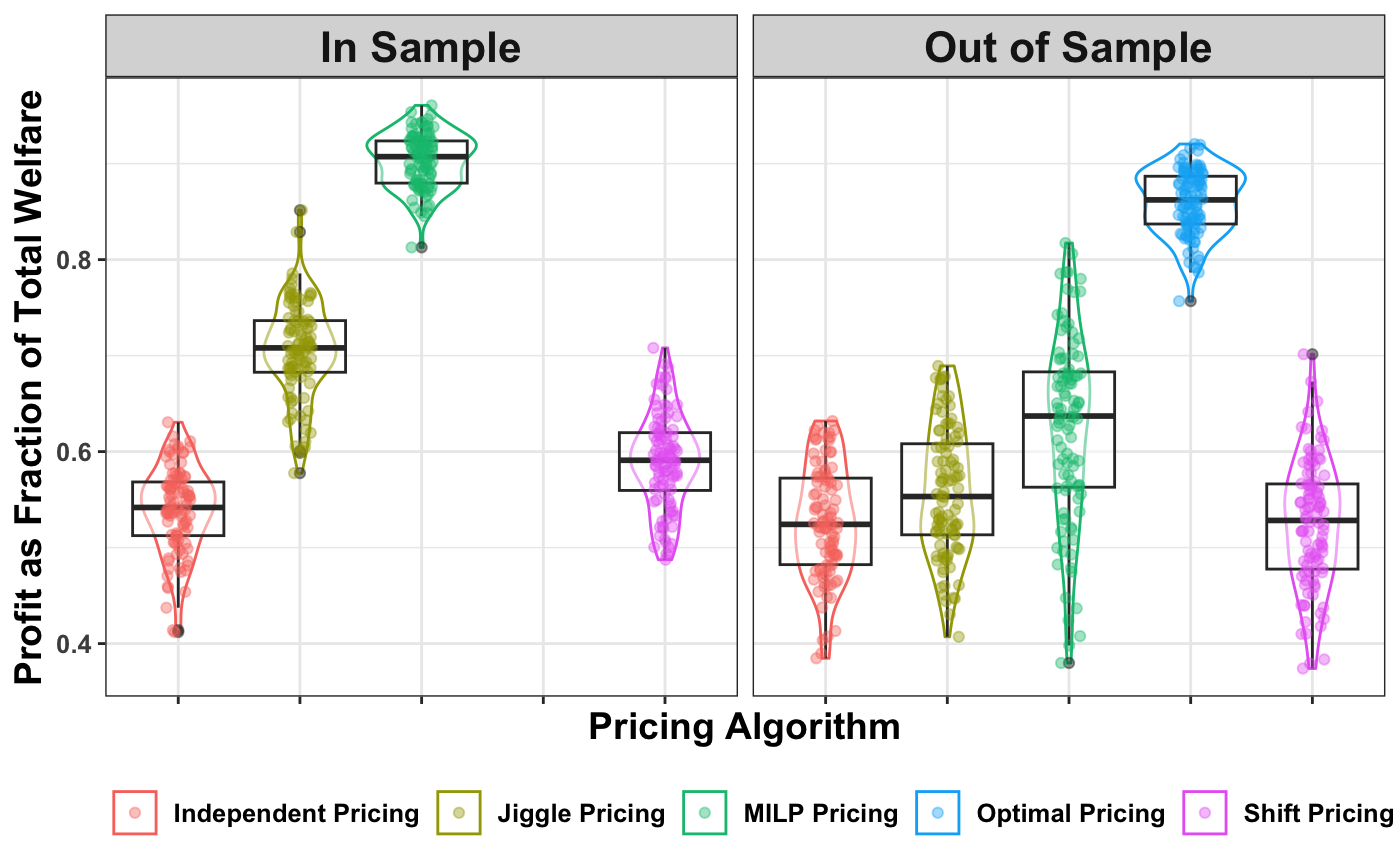
\includegraphics[width=\linewidth]{paper_rq1_figure3.png}
  \end{columns}
  \begin{alertblock}{结论}
    Data-Bandit 在相同搜索时间下更快获得高质量增强--模型组合。
  \end{alertblock}
\end{frame}

\begin{frame}{RQ1：复现实验}

\begin{columns}[T,onlytextwidth]
    \footnotesize
    \column{0.47\textwidth}
    \begin{block}{数据与搜索空间}
    \begin{itemize}
    \item UCI Wine Quality 数据，分类与回归各 30 个任务
    \item 2 个基础特征 + 9 个外部增强
        \item 6 个简单候选模型：线性/二次/随机ReLU Ridge
        \end{itemize}
        \end{block}
    \begin{exampleblock}{发现结果}
    \small
    \begin{itemize}
    \item Data-Bandit 前期效用曲线上升较快
        \item 同时由于模型简单，Alt的效用也不错
        \end{itemize}
        \end{exampleblock}
    \column{0.48\textwidth}
    \vspace{3em}
    \centering
    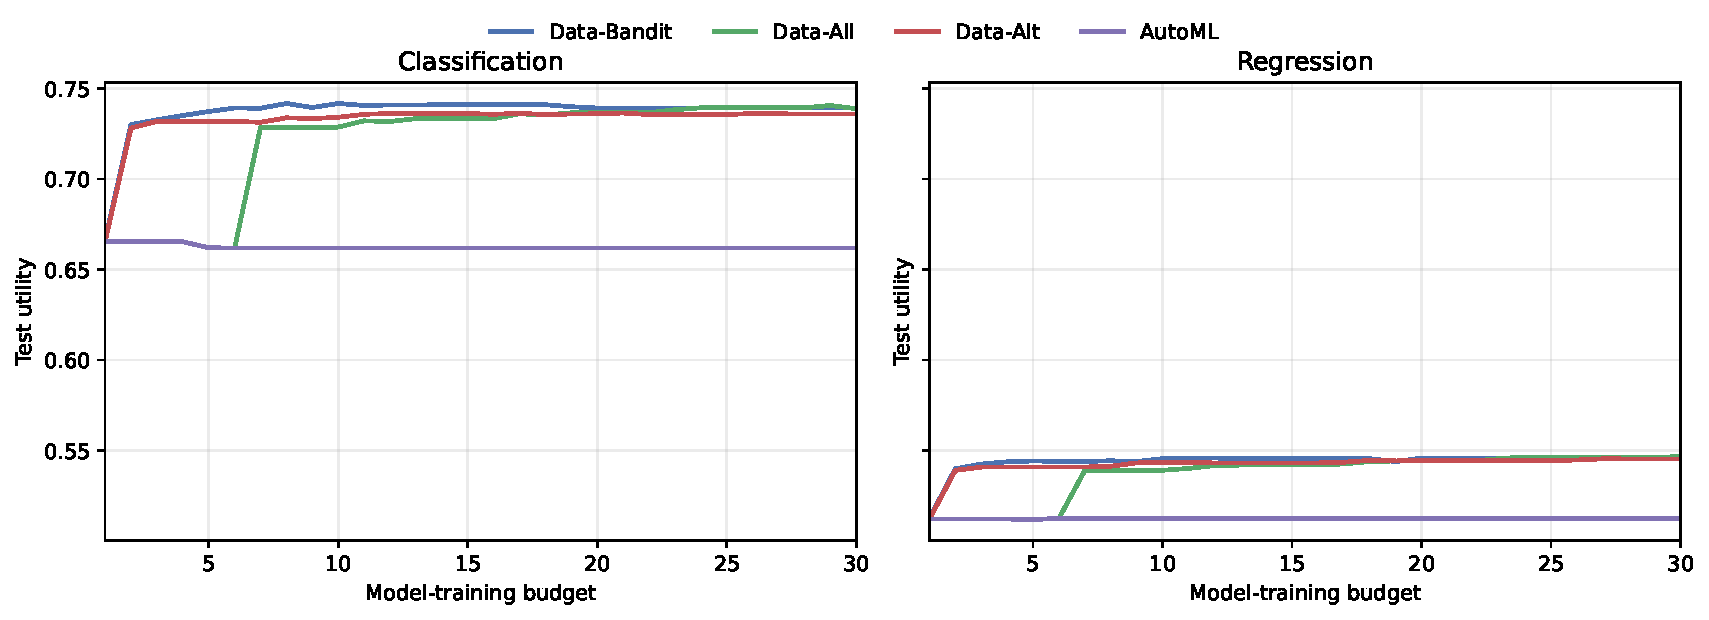
\includegraphics[width=1\linewidth]{rq1_discovery.pdf}
    \end{columns}
    \begin{alertblock}{复现边界}
      NYC 数据池、Metam 配置和完整代码未公开;Random Forest等模型耗时较长
    \end{alertblock}
  \vspace{0.2em}
\end{frame}

% ============================== RQ3 ==============================

\section{RQ3：先验学习}

\begin{frame}{RQ3：研究问题}
  \begin{columns}[T,onlytextwidth]
    \column{0.50\textwidth}
    \begin{block}{研究问题}
      平台未知买家类型先验时，能否仅凭停止轮次学习真实分布 $\mu^*$？
    \end{block}
    \begin{block}{观测变量}
      买家在给定价格曲线与搜索过程下的停止轮次 $Y$。
    \end{block}
    \column{0.45\textwidth}
    \begin{block}{评价指标}
      \begin{itemize}
        \item $D_{\rm KL}(\mu^*\|\mu^{(t)})$
        \item 学习率对收敛速度的影响
        \item 批量对估计稳定性的影响
      \end{itemize}
    \end{block}
    \begin{alertblock}{识别条件}
      观察不同买家类型产生可区分的停止分布
      \end{alertblock}
      \end{columns}
\end{frame}

\begin{frame}{RQ3：Algorithm 1 —— 平滑贝叶斯学习}
  \begin{columns}[T,onlytextwidth]
    \column{0.52\textwidth}
    \begin{block}{算法步骤}
      \begin{enumerate}
        \item 对每类 $\theta_i$ 预计算停止似然
              \[
                L_i(y)=\Pr(Y=y\mid\theta_i,x);
              \]
        \item 观察停止轮次 $y^{(t)}$ 后做 Bayes 更新
              \[
                w_i^{(t)}=\frac{L_i(y^{(t)})\mu_i^{(t)}}{\sum_jL_j(y^{(t)})\mu_j^{(t)}};
              \]
        \item 用学习率平滑
              \[
                \mu^{(t+1)}=(1-\eta_t)\mu^{(t)}+\eta_t\bar w^{(t)}.
              \]
      \end{enumerate}
    \end{block}
    \column{0.43\textwidth}
    \begin{block}{比较维度}
      \begin{itemize}
        \item 真实先验 $\mu^*$ 的收敛性
        \item 学习率与收敛速度、波动
        \item 批量与估计稳定性
      \end{itemize}
    \end{block}
    \begin{alertblock}{理论前提}
      不同类型必须产生可区分的停止分布；否则只看停止轮次不可能区分它们。
    \end{alertblock}
    \end{columns}
\end{frame}

\begin{frame}{RQ3：原文实验设计}
  \centering
  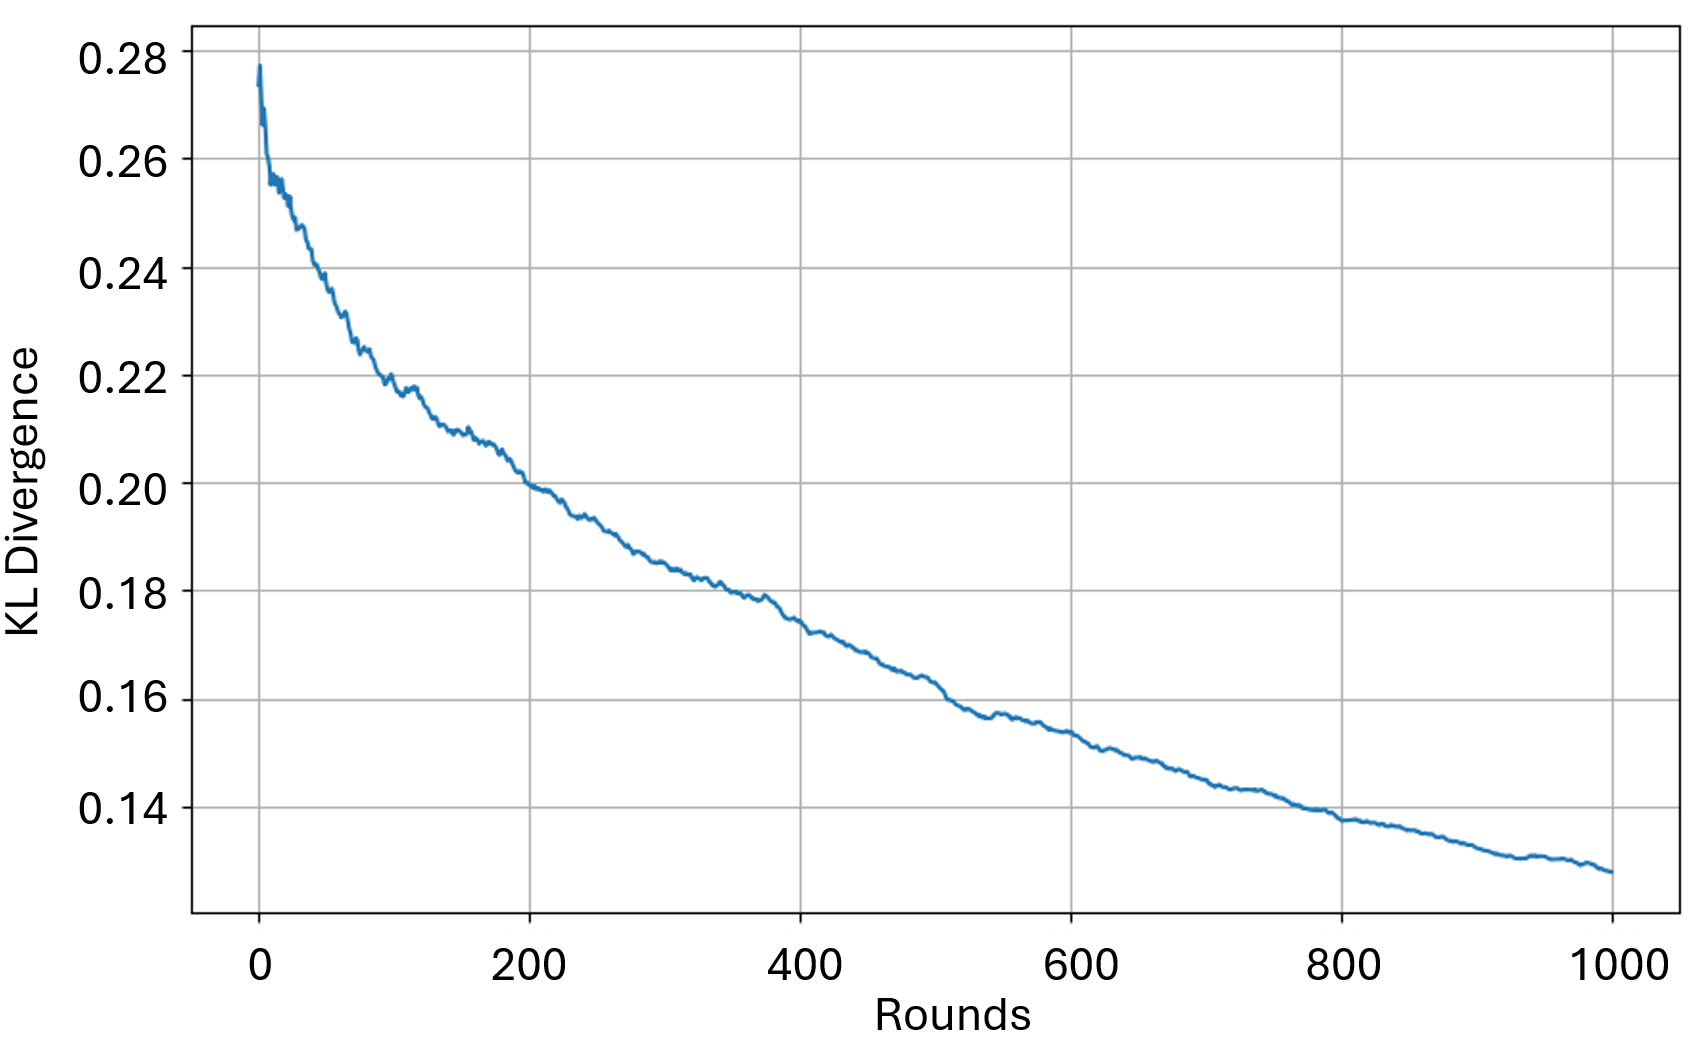
\includegraphics[width=0.26\linewidth]{paper_rq3_fig5_a.png}\hfill
  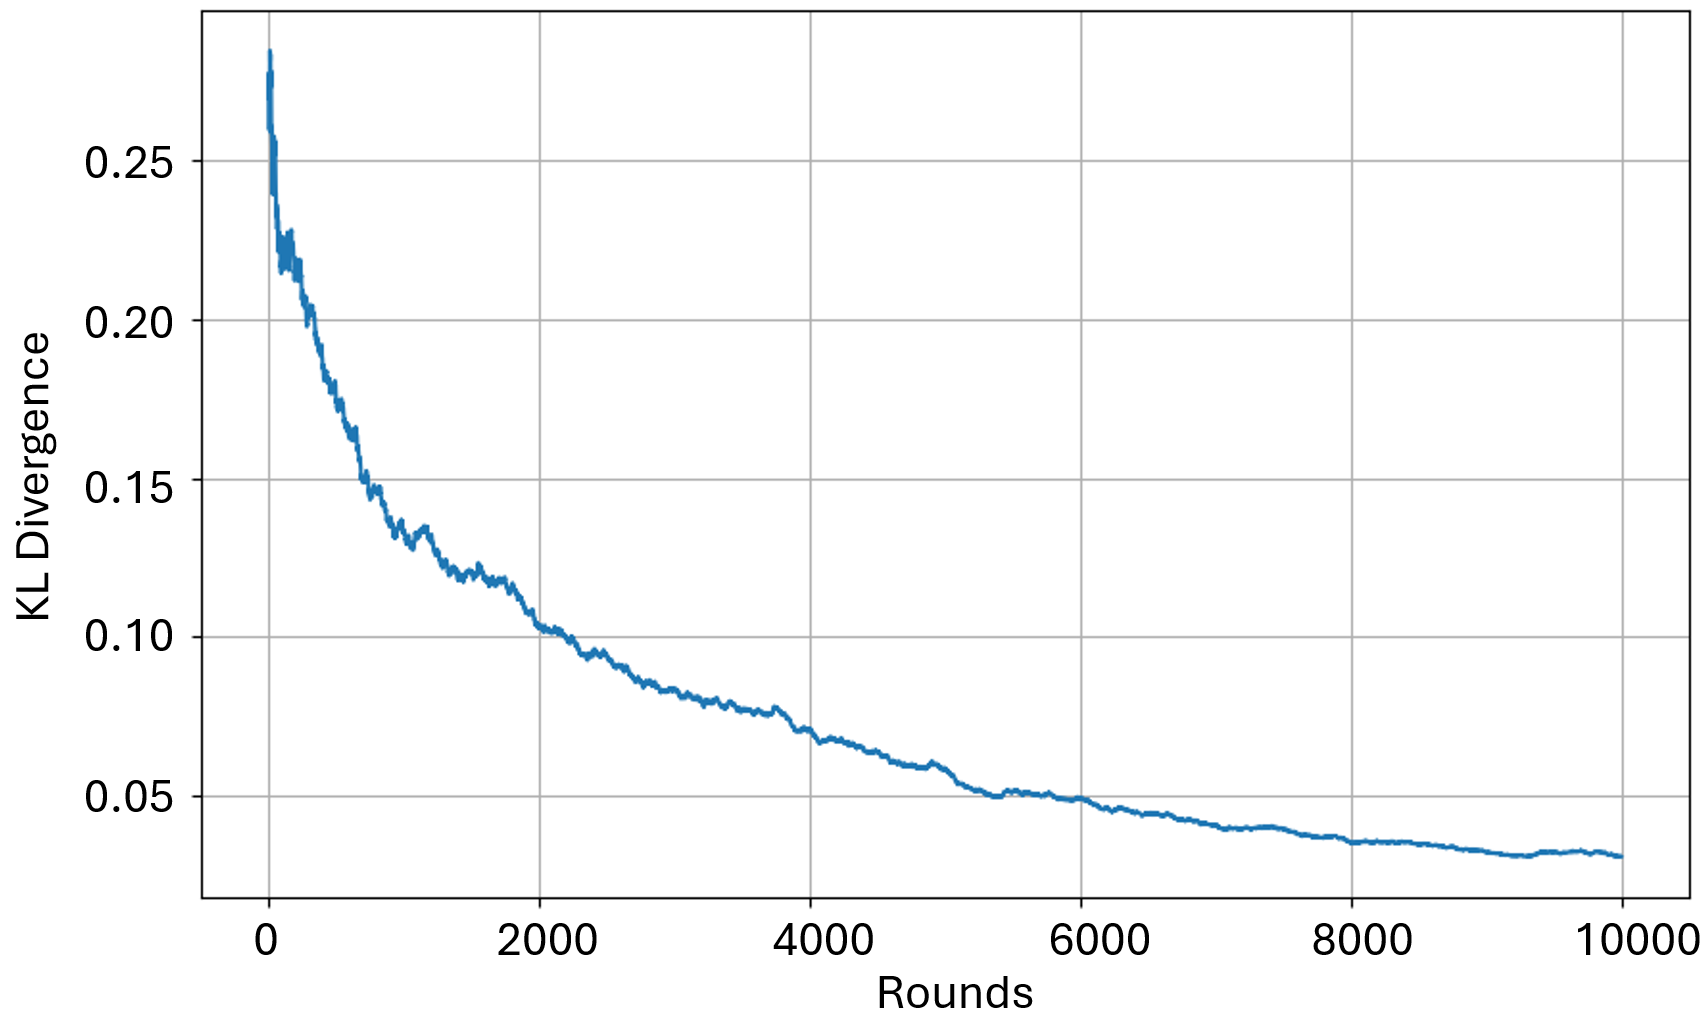
\includegraphics[width=0.26\linewidth]{paper_rq3_fig5_b.png}\hfill
  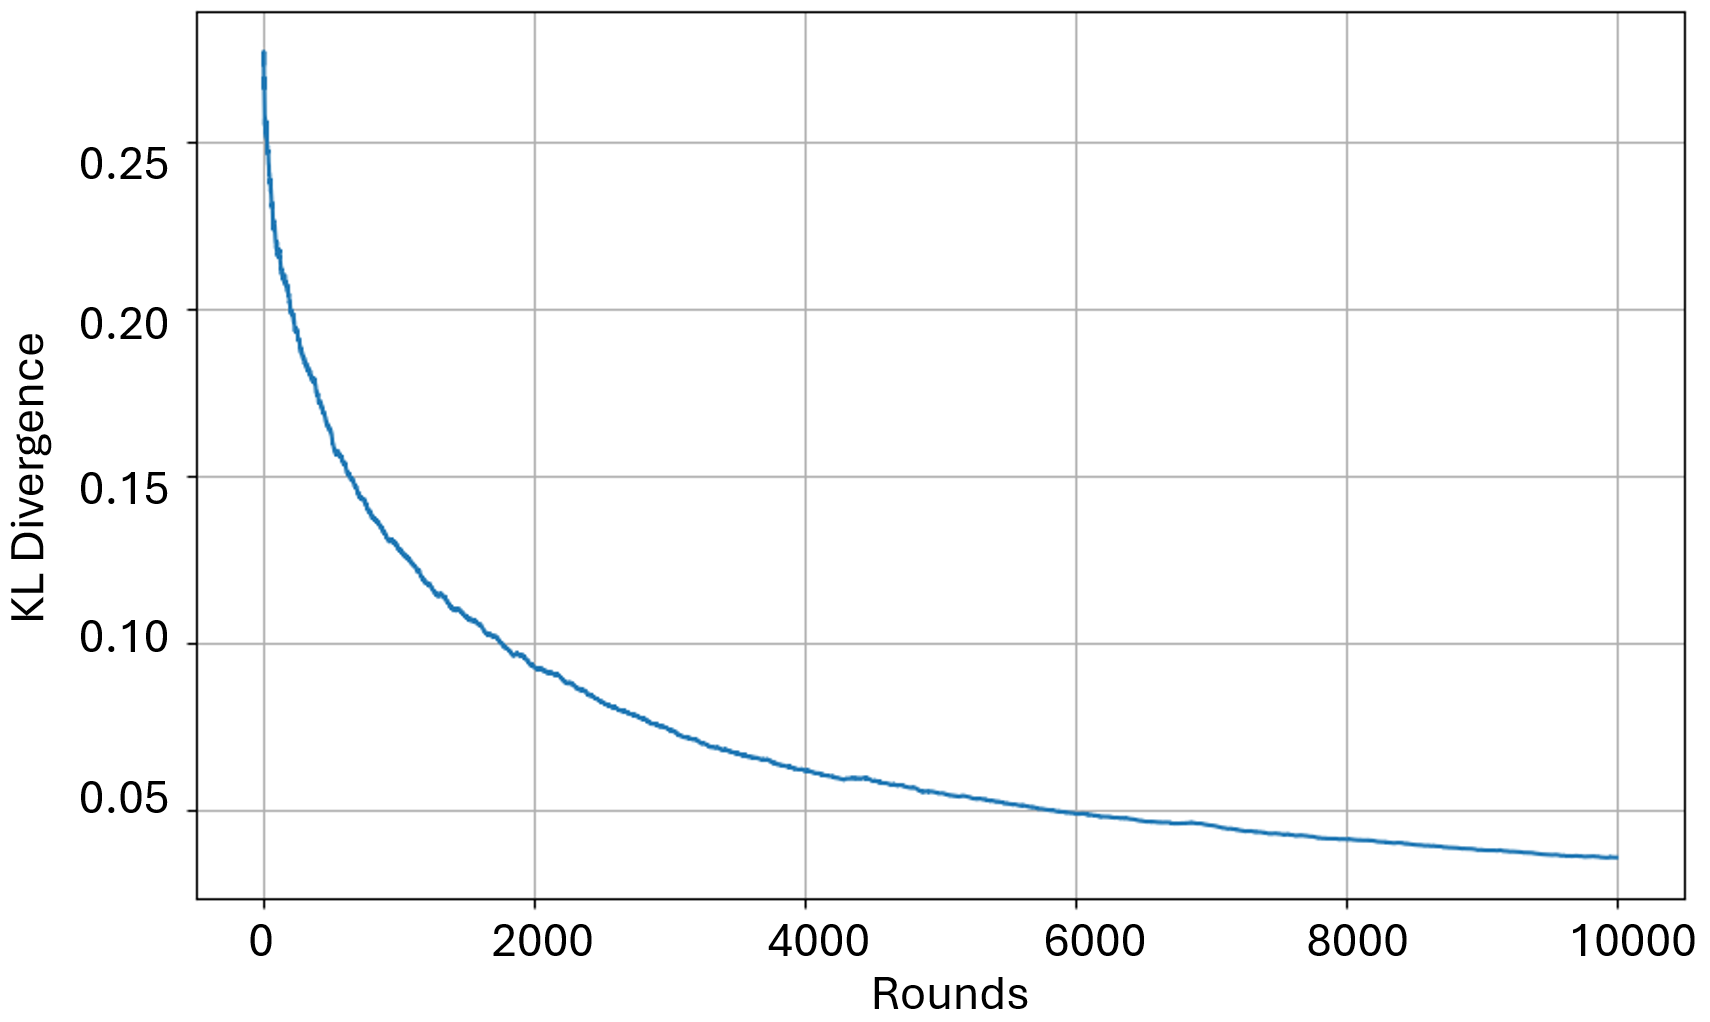
\includegraphics[width=0.26\linewidth]{paper_rq3_fig5_c.png}
  \\
  {\scriptsize Figure 5：固定 $\eta_t=1/\sqrt t$；(a) $b=100,N=1000$，(b) $b=10,N=10000$，(c) $b=100,N=10000$。}
  \begin{columns}[T,onlytextwidth]
    \column{0.50\textwidth}
    \begin{block}{论文模拟场景与设置}
    \scriptsize
    \begin{itemize}
        \item 性能档位 $\mathcal Q=\{100\%,\ldots,91\%\}$、搜索期限 $T=15$；真实先验 $\mu^*$ 随机生成
        \item 平台不观察买方类型，只观察其\key{停止轮次}，据此学习 $\mu^*$
        \item 正文 Figure 5 固定 $\eta_t=1/\sqrt t$，比较 $b=10/100$ 与学习轮数 $N$
        \item 另外$1/2$和$1/(t+1)$两种学习率见附录 Figure 6--7
        \end{itemize}
        \end{block}
    \column{0.45\textwidth}
    \begin{exampleblock}{结果分析}
    \scriptsize
    \begin{itemize}
    \item KL 散度随学习轮次下降
        \item Figure 5(b)(c)：同为 $N=10000$，$b=100$ 比 $b=10$ 平滑
        \item 较激进学习率收敛更快，但波动更大
        \end{itemize}
        \end{exampleblock}
        \end{columns}
  % \begin{alertblock}{原文结论}
  %   学习率与批量共同决定先验学习的收敛速度和稳定性。
  % \end{alertblock}
\end{frame}

\begin{frame}{RQ3：复现实验}
\centering

\includegraphics[height=0.42\textheight,keepaspectratio]{rq3_paper_reproduction.pdf}
\vspace{-0.45em}
\begin{columns}[T,onlytextwidth]
    \column{0.46\textwidth}
    \begin{block}{复现设置}
    \footnotesize
    \begin{itemize}
        \item 10 个质量状态、5 类估值、$T=15$；自行设定转移概率与成本
        \item 固定随机生成的五类买方占比；平台从均匀估计出发，初始 KL 为 0.2836
        \item 三种学习率、批量 10/100、5 个观测种子
        \item 前向 DP 计算似然
        \end{itemize}
        \end{block}
        \column{0.49\textwidth}
    \begin{alertblock}{复现结果分析}
    \footnotesize
    \begin{itemize}
        \item (a) 最终 KL：0.11952、0.02114、0.00497
        \item (b)(c) 同为 $N=10000$：$b=100$ 的收敛更平滑
        \item $1/(t+1)$ 最稳定但收敛慢；$1/2$ 前期快但振荡
        \item $1/\sqrt t$ 在大批量下兼顾下降速度与稳定性
        \item 原文未公开具体估值、转移过程、随机种子与代码
        \end{itemize}
        \end{alertblock}
        \end{columns}
  \vspace{-0.15em}
\end{frame}

% ============================== RQ2 ==============================

\section{RQ2：联合定价 MILP 的收入评估}

\begin{frame}{RQ2 核心问题}
  \begin{block}{核心问题}
    \key{联合定价 MILP} 相比传统基线能多收多少收入？IS 上训练的价格能否泛化到 OOS 新轨迹？
  \end{block}
  \vspace{0.6em}
  \begin{columns}[T,onlytextwidth]
    \begin{column}{0.48\textwidth}
      \begin{block}{Q1：MILP 是否优于简单方法？}
        \begin{itemize}
          \item 与 \key{Independent}、\key{Shift}、\key{Jiggle} 比较
          \item 评估跨质量联合定价的收入增量
        \end{itemize}
      \end{block}
    \end{column}
    \begin{column}{0.48\textwidth}
      \begin{block}{Q2：最优价格能否泛化？}
        \begin{itemize}
          \item IS 训练的价格 $\rightarrow$ OOS 测试
          \item 模拟真实部署中的分布外表现
        \end{itemize}
      \end{block}
    \end{column}
  \end{columns}
\end{frame}

\begin{frame}{实验设置：透明缩减的合成实例}
  \begin{block}{说明}
    本复现为\key{透明缩减设置}，非点对点复制。原文 School 数据任务和完整代码未公开，使用自包含合成数据。
  \end{block}
  \vspace{0.3em}
  \begin{columns}[T,onlytextwidth]
    \begin{column}{0.48\textwidth}
      \begin{block}{任务规格}
        \begin{itemize}
          \item 10 个随机重复任务
          \item 4 个离散质量状态
          \item 6 个异质买家类型
          \item 估值单调但增长率不同
        \end{itemize}
      \end{block}
    \end{column}
    \begin{column}{0.48\textwidth}
      \begin{block}{数据集与归一化}
        \begin{itemize}
          \item IS 训练：100 条全质量可达轨迹
          \item OOS 测试：4,000 条 Markov 随机轨迹
          \item 收入归一化：除以零价格期望福利
        \end{itemize}
      \end{block}
    \end{column}
  \end{columns}
\end{frame}

\begin{frame}{复现实现思路：四层架构，数据全部程序化生成}
  \begin{enumerate}
    \setlength{\itemsep}{0.6em}
    \item \key{合成市场构造}：\texttt{synthetic\_instance(seed)} 生成估值矩阵、Markov 转移矩阵与先验分布。全部硬编码 + 固定 seed，零外部数据依赖。
    \item \key{轨迹生成}：IS 轨迹由 \texttt{np.tile([0,1,2,3], (100,1))} 确定性构造；OOS 轨迹由 \texttt{simulate\_markov\_trajectories} 随机采样 4,000 条。
    \item \key{定价方法}：MILP 调用 HiGHS，Big-M 线性化 $y=x\cdot z$，bitmask 压缩相同 availability set。Independent / Shift / Jiggle 用估值网格穷举或局部搜索。
    \item \key{收入评估}：每种价格 $\times$ IS/OOS $\times$ forced/realized 共 4 个指标，10 次重复取 \good{均值 $\pm$ 标准误}。
  \end{enumerate}
\end{frame}

\begin{frame}{五种定价方法}
  \renewcommand{\arraystretch}{1.3}
  \begin{tabularx}{\linewidth}{>{\bfseries\color{ZJUBlue}}l c >{\raggedright\arraybackslash}X}
    \toprule
    方法 & 来源 & 思路 \\
    \midrule
    MILP (IS) & Theorem 4.2 & IS 轨迹上求解联合定价 MILP，最大化经验期望收入。\\
    Independent & Appendix D.1 & 逐质量垄断定价，忽略跨质量替代效应。\\
    Shift & Appendix D.1 & 从 Independent 出发，统一偏移所有质量的价格。\\
    Jiggle & Appendix D.1 & 从 Shift 初始解做贪心局部搜索直至收敛。\\
    OOS-MILP & 参考上界 & 直接使用 OOS 轨迹训练的 MILP，衡量 IS 信息损失。\\
    \bottomrule
  \end{tabularx}
  \vspace{0.4em}
  \begin{center}
    \key{排序预期}：Independent $\le$ Shift $\le$ Jiggle（不劣性链，Appendix D.1）
  \end{center}
\end{frame}

\begin{frame}{同一个 MILP，两种评价指标}
  \begin{columns}[T,onlytextwidth]
    \begin{column}{0.48\textwidth}
      \begin{block}{Forced-choice（论文指标）}
        \begin{itemize}
          \item 买家必须选择模型
          \item 即使净效用为负也必须买
          \item $\rightarrow$ MILP 直接优化的目标
        \end{itemize}
        \centering
        \large\good{IS 归一化收入：0.7926}
      \end{block}
    \end{column}
    \begin{column}{0.48\textwidth}
      \begin{block}{Realized（自愿购买）}
        \begin{itemize}
          \item 买家有不购买选项
          \item 净效用为负 $\rightarrow$ 退出
          \item $\rightarrow$ 真实市场可实现的收入
        \end{itemize}
        \centering
        \large\good{OOS 实现收入：0.4075}
      \end{block}
    \end{column}
  \end{columns}
  \vspace{0.5em}
  \begin{block}{关键差异}
    \key{从 0.79 跌到 0.41——近一半收入因买家退出而消失。}
    评价语义的选择会根本性地改变方法排序。这不是论文错了，而是理解本文最重要的 nuance。
  \end{block}
\end{frame}

\begin{frame}{核心数值结果：Forced-choice 指标}
  \begin{columns}[c,onlytextwidth]
    \begin{column}{0.52\textwidth}
      \centering
      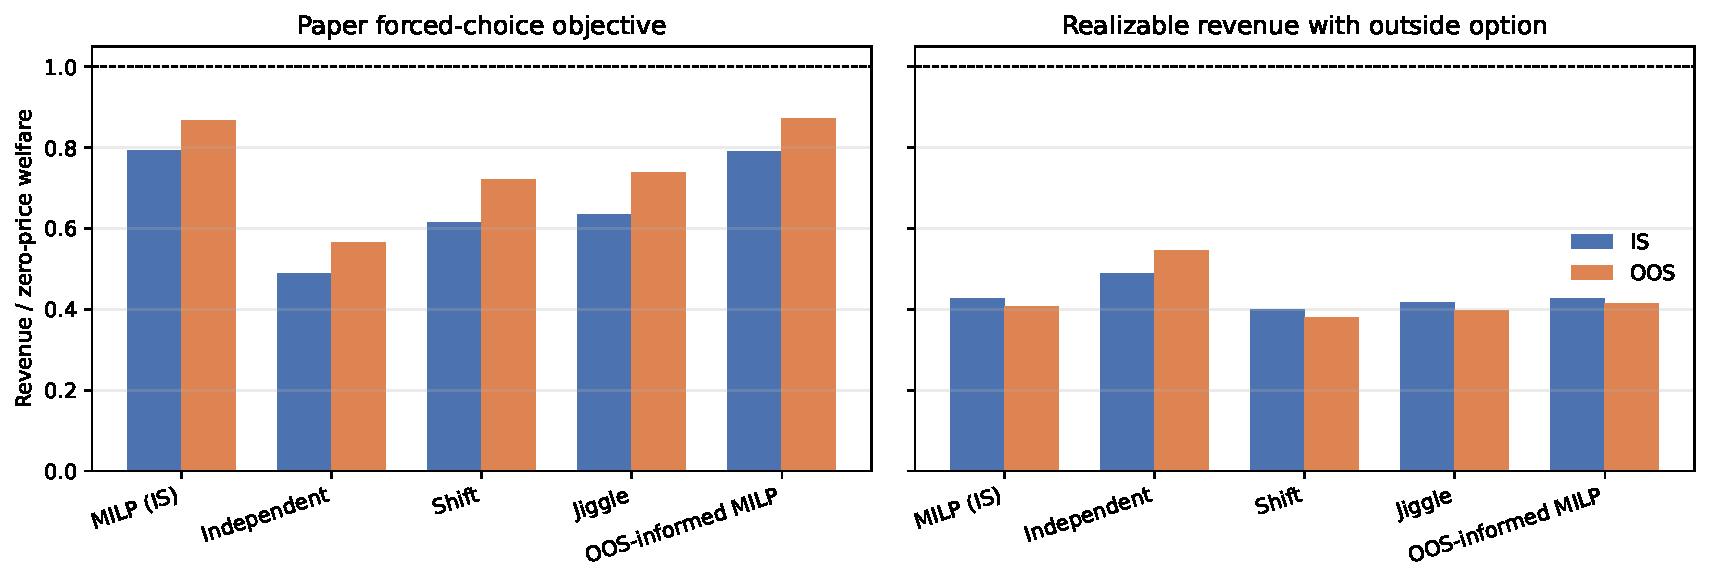
\includegraphics[width=\linewidth]{rq2_paper_reproduction.pdf}
    \end{column}
    \begin{column}{0.44\textwidth}
      \begin{block}{方法排序（符合论文预期）}
        \small
        \begin{tabularx}{\linewidth}{>{\bfseries\color{ZJUBlue}}X c}
          \toprule
          方法 & 归一化收入 \\
          \midrule
          \good{MILP (IS)} & \good{0.7926 $\pm$ 0.0098} \\
          OOS-Informed MILP & 0.7898 \\
          Jiggle & 0.6353 \\
          Shift & 0.6157 \\
          Independent & 0.4880 \\
          \bottomrule
        \end{tabularx}
      \end{block}
      \vspace{0.3em}
      \key{结论}：MILP 捕获约 79\% 零价格福利；原文 Fig.\ 4 约 85\%，差距合理。不劣性链成立。
    \end{column}
  \end{columns}
\end{frame}

\begin{frame}{核心数值结果：自愿购买指标——排序翻转}
  \begin{columns}[T,onlytextwidth]
    \begin{column}{0.48\textwidth}
      \begin{block}{OOS Realized 收入排序}
        \begin{tabular}{lc}
          \toprule
          方法 & 归一化收入 \\
          \midrule
          \good{Independent} & \good{0.5468 $\pm$ 0.0119} \\
          IS MILP & 0.4075 $\pm$ 0.0138 \\
          Shift & $\sim$0.38 \\
          Jiggle & $\sim$0.38 \\
          \bottomrule
        \end{tabular}
      \end{block}
    \end{column}
    \begin{column}{0.48\textwidth}
      \begin{block}{为什么 Independent 反而最好？}
        \begin{itemize}
          \item 逐质量独立定价，不推高整体价格曲线
          \item MILP 统一定高价收割高估值买家$\rightarrow$有退出后大量流失
        \end{itemize}
      \end{block}
      \key{正确解读}：不是 Independent 普遍最优，而是论文优化目标 $\neq$ 真实购买行为，两者之间存在语义边界。
    \end{column}
  \end{columns}
\end{frame}

\section{改进方案}

\begin{frame}{复现中发现的四个机制问题}
\begin{enumerate}
\setlength{\itemsep}{0.5em}
\item \key{强制购买不现实。}
论文 MILP 约束每个买家必须购买。实验显示：加入退出选项后，论文最优价格的实际收入从 $0.79$ 跌至 $0.41$——近一半收入消失，方法排序完全翻转。

\item \key{冷启动矛盾。}
定价需要已知买家分布 $\mu$，但 $\mu$ 又需要多轮交易才能学到——第一轮价格凭什么最优？

    \item \key{搜索成本被忽略。}
    定理 4.2 假设 $c\approx0$。但 $c>0$ 时买家会更早停止、看到更少选项，最优价格应与搜索成本耦合。

    \item \key{定价与发现过程脱节。}
    论文把"发现什么增强"和"怎么定价"当作独立模块。但发现引擎的轨迹分布直接影响买家选择——平台应根据定价目标引导发现方向。
    \end{enumerate}
\end{frame}

\begin{frame}{四个改进方向}
\renewcommand{\arraystretch}{1.35}
\begin{tabularx}{\linewidth}{>{\bfseries\color{ZJUBlue}}l >{\raggedright\arraybackslash}X}
  \toprule
  改进                 & 思路                                                    \\
  \midrule
  \good{IR-aware 定价} & 把退出权利写进 MILP 目标函数，定价时就考虑"买家可以不买"。代码已有原型。              \\
  \good{鲁棒定价}        & 分布鲁棒优化，让价格在最坏先验下也有保障，随数据增多逐步收敛。                       \\
  \good{成本感知定价}      & 解除 $c\approx0$ 假设，推导搜索成本非零时的修正 MILP。精确 Markov 评估器已就绪。 \\
  \good{定价引导发现}      & 把价格信号反馈给 Data-Bandit，优先探索高收入潜力的增强方向。                  \\
  \bottomrule
\end{tabularx}
\vspace{0.6em}
\begin{alertblock}{预期贡献}
从"强制购买、先验已知、成本忽略、发现定价割裂"的理想模型，推向更贴近真实市场的完整机制。
  \end{alertblock}
\end{frame}

\begin{frame}[allowframebreaks]{参考文献}
  \nocite{*}
  \bibliographystyle{unsrt}
  \bibliography{references}
\end{frame}

\end{document}
